

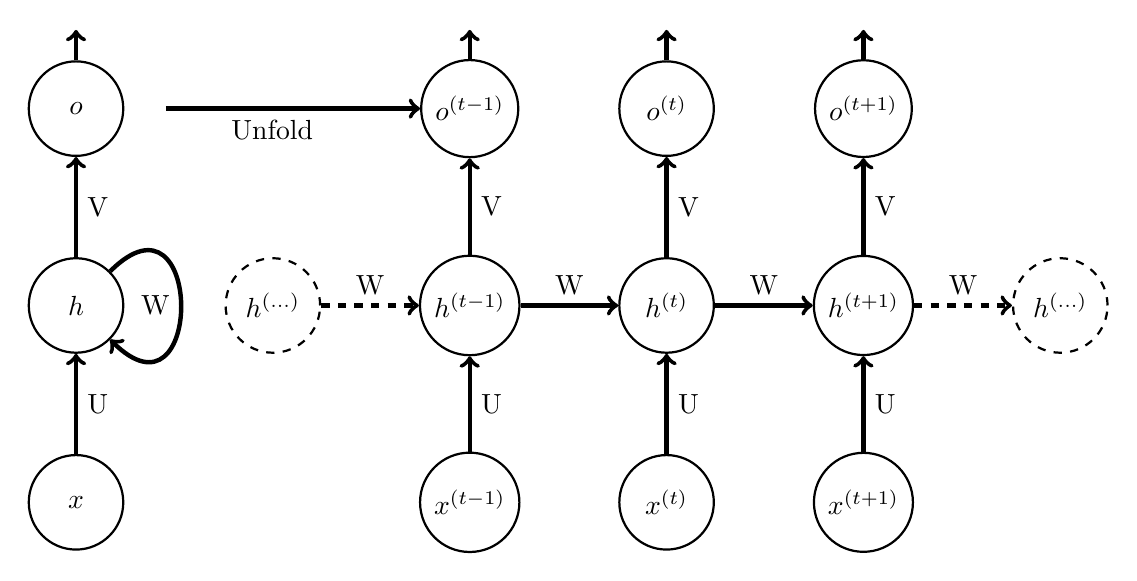
\begin{tikzpicture}[
    node distance = 25mm,
    thick,
    main/.style = {draw, circle, minimum size = 1.2cm}
]

% Base nodes
\node[main] (1) {$x$};
\node[main] (2) [above of=1] {$h$};
\node[main] (3) [above of=2] {$o$};

% Time-unfolded hidden states
\node[main, dashed] (4) [right of=2] {$h^{(...)}$};
\node[main]          (5) [right of=4] {$h^{(t-1)}$};
\node[main]          (6) [right of=5] {$h^{(t)}$};
\node[main]          (7) [right of=6] {$h^{(t+1)}$};
\node[main, dashed] (8) [right of=7] {$h^{(...)}$};

% Outputs
\node[main] (9)  [above of=5] {$o^{(t-1)}$};
\node[main] (10) [above of=6] {$o^{(t)}$};
\node[main] (11) [above of=7] {$o^{(t+1)}$};

% Inputs
\node[main] (12) [below of=5] {$x^{(t-1)}$};
\node[main] (13) [below of=6] {$x^{(t)}$};
\node[main] (14) [below of=7] {$x^{(t+1)}$};

% Recurrent and input/output connections
\draw[ultra thick, ->] (2) to [out=45, in=315, looseness=5] node[left] {W} (2);
\draw[ultra thick, ->] (1)  -- node[right] {U} (2);
\draw[ultra thick, ->] (2)  -- node[right] {V} (3);

\draw[ultra thick, ->, dashed] (4) -- node[above] {W} (5);
\draw[ultra thick, ->]         (5) -- node[above] {W} (6);
\draw[ultra thick, ->]         (6) -- node[above] {W} (7);
\draw[ultra thick, ->, dashed] (7) -- node[above] {W} (8);

\draw[ultra thick, ->] (12) -- node[right] {U} (5);
\draw[ultra thick, ->] (13) -- node[right] {U} (6);
\draw[ultra thick, ->] (14) -- node[right] {U} (7);

\draw[ultra thick, ->] (5) -- node[right] {V} (9);
\draw[ultra thick, ->] (6) -- node[right] {V} (10);
\draw[ultra thick, ->] (7) -- node[right] {V} (11);

% Output arrows
\draw[ultra thick, ->] (9)  -- +(0,1);
\draw[ultra thick, ->] (10) -- +(0,1);
\draw[ultra thick, ->] (11) -- +(0,1);
\draw[ultra thick, ->] (3)  -- +(0,1);

% Unfold arrow
\draw[ultra thick, ->, shorten <=15pt] 
    (3) -- node[below]{Unfold} ([xshift=-40pt]9);

\end{tikzpicture}

\vspace{5pt}


